% !TEX encoding = UTF-8 Unicode
\subsection{Fase PROP: Progettazione Requisiti Opzionali}
	\textbf{Periodo}: dal \insdate{19}{04}{2015} al \insdate{07}{05}{2015} \\Questa fase comincia subito dopo la scadenza della consegna per la \insrev{Revisione di Progetto} e termina con l'incontro con il proponente al fine di mostrare il prototipo con tutti i requisiti (obbligatori, desiderabili e opzionali) sviluppati. 
	\\Le attività di questa fase saranno le seguenti:
	\begin{itemize}
		\item\textbf{Definizione di Prodotto}: viene steso il documento \insdoc{Definizione di Prodotto v3.0}. Esso definisce la struttura interna del sistema e le relazioni dei componenti del prodotto relativi ai requisiti opzionali.
		\item \textbf{Codifica}: con quest'attività inizia lo sviluppo da parte dei programmatori dei requisiti opzionali. Sarà dunque seguito quanto riportato nel documento \insdoc{Definizione di Prodotto v3.00};
		\item \textbf{Esecuzione test}: verranno eseguiti automaticamente tutti i test di unità e integrazione previsti dal documento \insdoc{Piano di Qualifica v 6.00};
		\item\textbf{Manuale Utente e Manuale Amministratore}: comincia la stesura dei manuali che forniranno indicazioni agli utilizzatori del sistema.
		\item\textbf{Incremento e Verifica Documenti}: vengono eseguite modifiche ai documenti già scritti, se necessario.
		\item\textbf{Glossario}: vengono aggiunti al file \insfile{Glossario.xml} i vocaboli dei quali si ritiene necessaria una definizione formale. Alla fine di questa fase vieni quindi generato il documento \insdoc{Glossario v6.00}.
	\end{itemize}
	\subsubsection{Diagramma di Gantt delle attività}
	\begin{figure}[H]\centering
		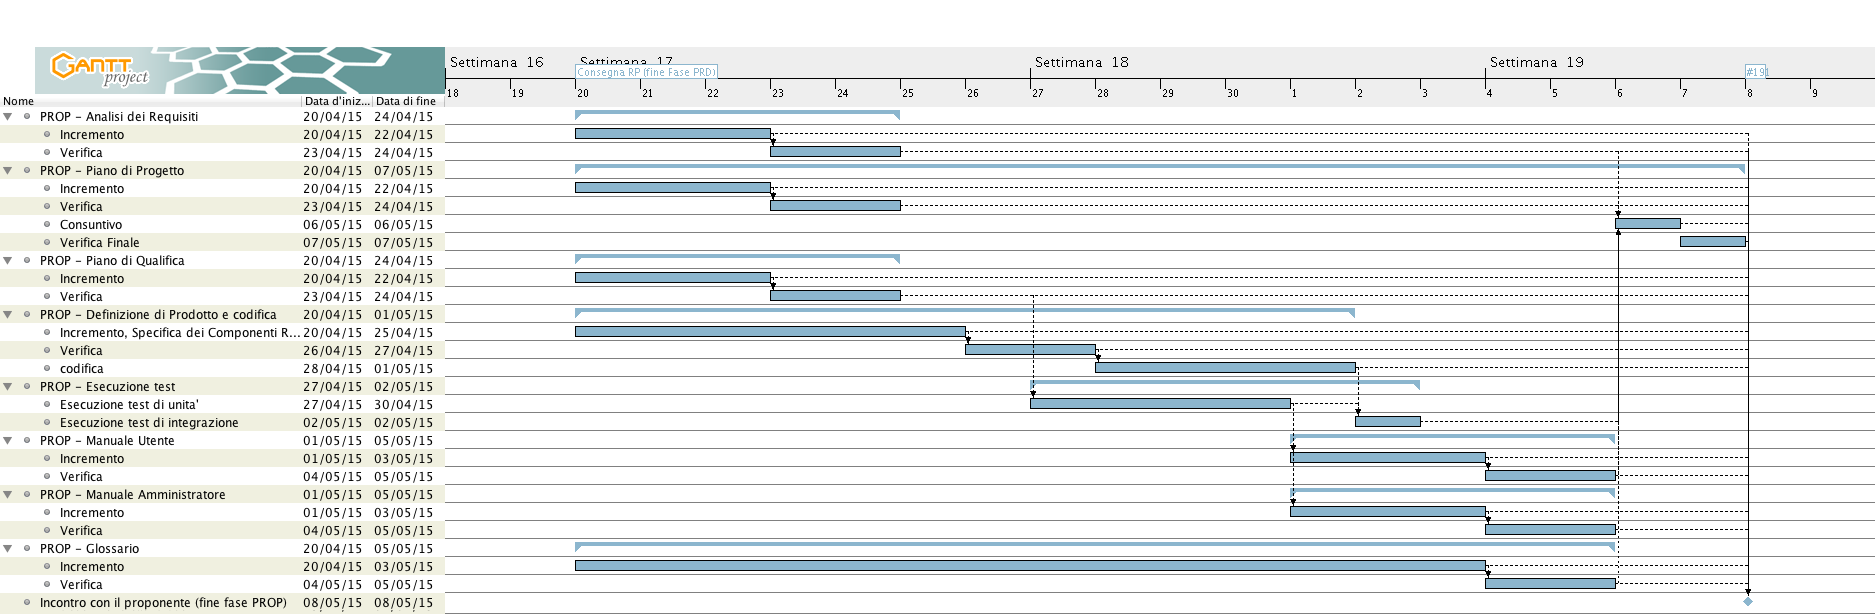
\includegraphics[width=\textwidth]{PianoDiProgetto/Pics/FasePROP.png}
	\caption{Gantt Fase PROP}
\end{figure}